\section{Introducción}

El phishing sigue siendo una de las amenazas más frecuentes en Internet: solo en el segundo trimestre de 2026, el Anti-Phishing Working Group registró 1.069.681 ataques, un 10,1~\% más que el trimestre anterior~\cite{apwg2026}. La mayoría de estos ataques llega como un enlace a un sitio que imita a una marca conocida, por lo que clasificar la URL antes de que el usuario la abra es una defensa rápida y que no requiere visitar el sitio sospechoso~\cite{ma2009,sahingoz2019}.

Los trabajos recientes reportan exactitudes sobre 99~\% en datasets públicos~\cite{prasad2024,dubey2025}. Sin embargo, un desempeño casi perfecto puede deberse a \emph{atajos}: patrones que separan las clases por cómo se construyó el dataset y no por las propiedades del fenómeno~\cite{geirhos2020}. En seguridad, este problema de correlaciones espurias es uno de los errores más comunes al aplicar aprendizaje automático~\cite{arp2022}.

El objetivo de este trabajo es comparar modelos de Machine Learning y Deep Learning para detectar URLs de phishing en el dataset PhiUSIIL~\cite{prasad2024} y medir cuánto de su desempeño se explica por atajos. Las contribuciones son: (i) la identificación de tres atajos en PhiUSIIL; (ii) la comparación de cuatro modelos tabulares en cuatro escenarios y de tres modelos de texto con tres entradas distintas; y (iii) una estimación del desempeño sin atajos, usando solo el dominio. El código y los resultados se encuentran en un repositorio público\footnote{\url{https://github.com/54isaac09/Machine-Learning-phishing-url-detection}}.

\section{Trabajos relacionados}

Ma et al.~\cite{ma2009} mostraron que las características léxicas y de host de una URL bastan para detectar sitios maliciosos con modelos lineales. Sahingoz et al.~\cite{sahingoz2019} compararon siete clasificadores con características de procesamiento de lenguaje natural y obtuvieron los mejores resultados con Random Forest. Otra línea evita la ingeniería de características: URLNet~\cite{le2018} aprende representaciones de caracteres y palabras con redes convolucionales, y Aljofey et al.~\cite{aljofey2020} propusieron una CNN de caracteres que solo usa la URL. Dubey et al.~\cite{dubey2025} combinaron una CNN de caracteres con LightGBM en un ensamble.

Prasad y Chandra~\cite{prasad2024} publicaron PhiUSIIL junto con un marco basado en un índice de similitud con URLs legítimas y aprendizaje incremental. En cuanto a la validez de estas evaluaciones, Mia et al.~\cite{mia2024} mostraron con SHAP que la importancia de las características cambia entre datasets y que el desempeño cae al evaluar en un dataset distinto al de entrenamiento. Este trabajo se apoya en las recomendaciones de Arp et al.~\cite{arp2022} y en el marco de aprendizaje por atajos de Geirhos et al.~\cite{geirhos2020} para analizar PhiUSIIL.

\section{Datos}

\subsection{Dataset}
PhiUSIIL contiene 235.795 URLs (134.850 legítimas y 100.945 de phishing) con 50 variables numéricas y 4 de texto (URL, dominio, TLD y título de la página)~\cite{prasad2024}. No tiene valores faltantes. Se eliminaron 425 URLs duplicadas, todas con etiquetas consistentes, y quedaron 235.370. En el archivo original la etiqueta vale 1 para las legítimas; se creó la variable \texttt{es\_phishing} para que la clase positiva sea phishing.

Las variables numéricas se agruparon según lo que requieren: 21 se calculan solo con el texto de la URL, 28 requieren descargar y analizar el HTML de la página y una, \texttt{URLSimilarityIndex}, compara la URL con una lista de URLs legítimas.

\subsection{Análisis exploratorio y atajos}
El AUC univariado de \texttt{URLSimilarityIndex} es 0,996, y seis variables de la página superan 0,95. Al investigar este resultado se encontraron los tres patrones de la Tabla~\ref{tab:atajos} y la Fig.~\ref{fig:atajos}: todas las URLs legítimas comienzan con \texttt{https://www.}, ninguna tiene ruta y todas tienen \texttt{URLSimilarityIndex} = 100. Esto se explica porque las legítimas provienen de listas de dominios populares escritas con un mismo formato, mientras que las de phishing son enlaces reales completos. Un modelo puede, por lo tanto, separar las clases sin aprender nada sobre el phishing.

\begin{table}[t]
\caption{Atajos detectados en PhiUSIIL (porcentaje de cada clase)}
\label{tab:atajos}
\centering
\begin{tabular}{lrr}
\toprule
Patrón & Legítimas & Phishing \\
\midrule
\texttt{URLSimilarityIndex} = 100 & 100,0 & 0,8 \\
Comienza con \texttt{https://www.} & 100,0 & 2,4 \\
Tiene ruta después del dominio & 0,0 & 59,7 \\
\texttt{IsHTTPS} = 1 & 100,0 & 49,1 \\
\bottomrule
\end{tabular}
\end{table}

\begin{figure}[t]
\centering
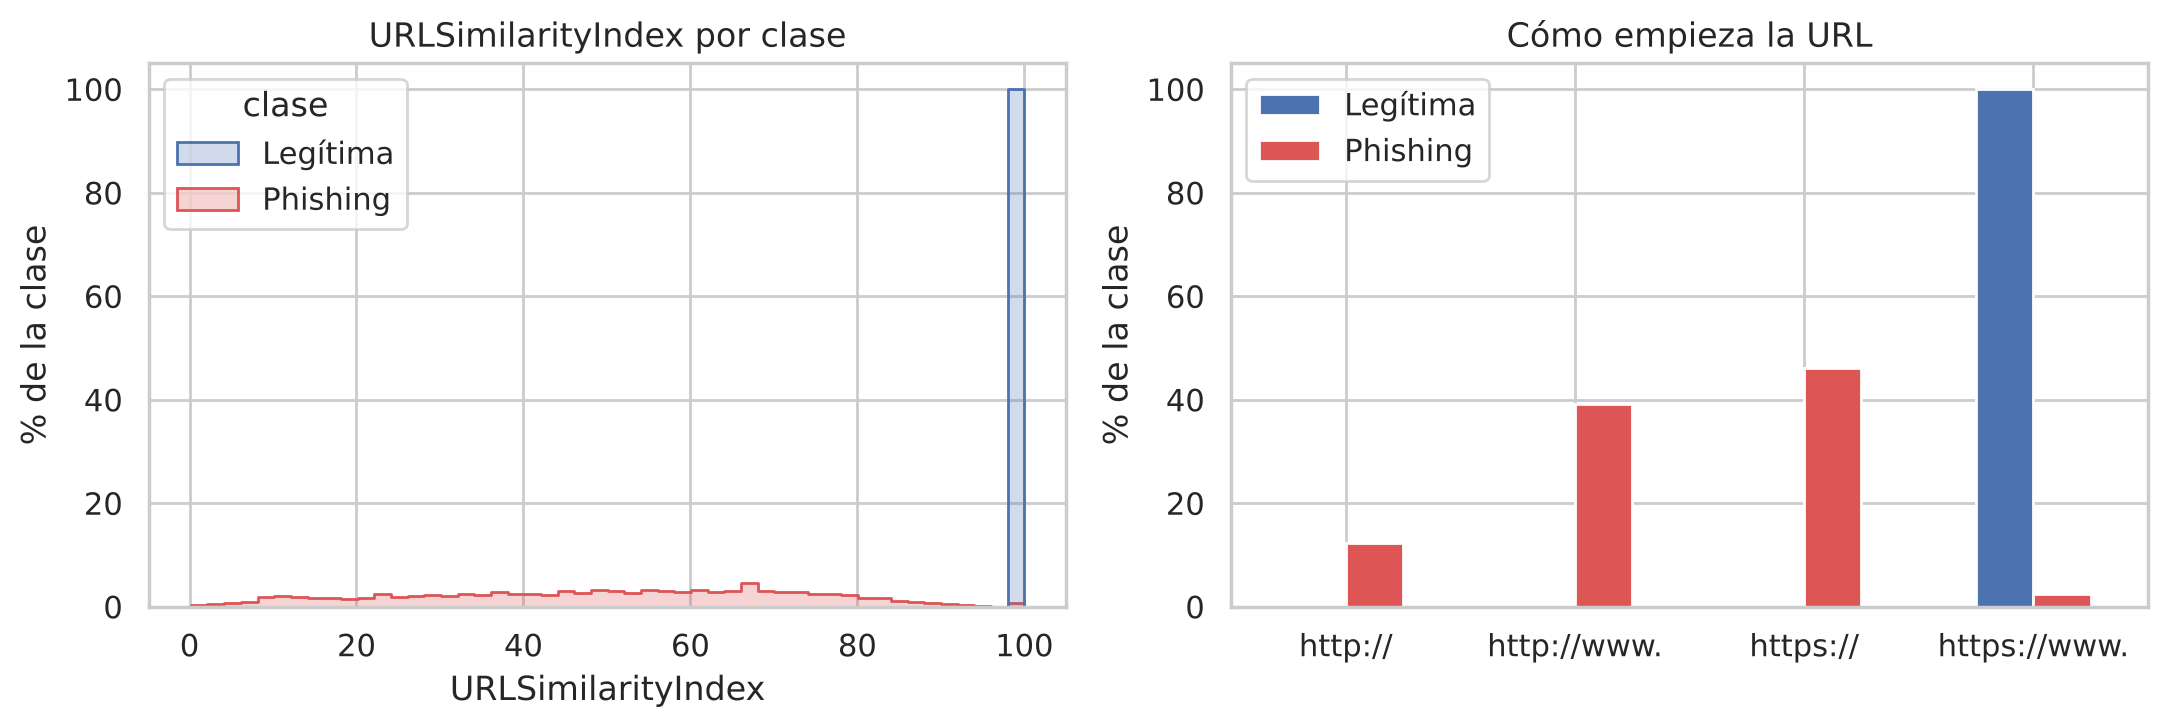
\includegraphics[width=\columnwidth]{03_atajos.png}
\caption{Distribución de \texttt{URLSimilarityIndex} y del prefijo de la URL por clase.}
\label{fig:atajos}
\end{figure}

\subsection{División de los datos}
Muchas URLs de phishing comparten dominio (por ejemplo, 1.192 URLs en \texttt{ipfs.io}). Para evitar que un modelo reconozca dominios ya vistos, la división en entrenamiento, validación y prueba (70/15/15~\%) se hizo agrupando por dominio: 164.918, 35.206 y 35.246 URLs, con cerca de 42~\% de phishing en cada conjunto. La validación se usó para comparar y ajustar modelos, y el conjunto de prueba se usó una sola vez al final.

\section{Metodología}

\subsection{Enfoque A: modelos tabulares}
Se compararon regresión logística, Random Forest (150 árboles), XGBoost~\cite{chen2016} y un perceptrón multicapa (capas de 64 y 32 neuronas). Para la regresión logística y el perceptrón, las variables se transformaron con $\log(1+x)$ y se estandarizaron. Se definieron cuatro escenarios, de más a menos atajos: A1, las 50 variables; A2, sin \texttt{URLSimilarityIndex}; A3, solo las 21 variables de la URL; y A4, 46 variables léxicas propias calculadas únicamente con el dominio (largo, puntos, guiones, dígitos, proporción de vocales, entropía de Shannon, palabras como \emph{login} o \emph{secure} y TLD). Los hiperparámetros de XGBoost en A4 se ajustaron con una grilla de 12 combinaciones de profundidad, tasa de aprendizaje y peso mínimo por hoja, con detención temprana en validación.

\subsection{Enfoque B: modelos de texto}
Los modelos de texto reciben tres entradas: la URL original, la URL normalizada (sin esquema, sin \texttt{www.} y sin la barra final) y solo el dominio. Se compararon: (i) TF-IDF de n-gramas de 2 a 4 caracteres (100.000 términos) con regresión logística; (ii) una CNN de caracteres con \emph{embedding} de 32 dimensiones, filtros convolucionales de anchos 2 a 5 (64 por ancho), \emph{global max pooling}, una capa densa de 64 neuronas y \emph{dropout} de 0,3; y (iii) una BiGRU de 32 unidades por dirección. Las redes se entrenaron en Keras con Adam (tasa $10^{-3}$), entropía cruzada binaria, lotes de 256 y detención temprana (paciencia 3, máximo 25 épocas). El dominio se truncó a 64 caracteres y la URL a 128.

\subsection{Evaluación}
La clase positiva es phishing. Se reportan precisión, \emph{recall}, F1 y ROC-AUC. Para cada escenario se seleccionó el modelo con mayor F1 en validación. Las predicciones de XGBoost se explicaron con SHAP~\cite{lundberg2017}.
